% ==========================================================
%  OLD EXAM QUESTIONS — Computer Vision
% ==========================================================

\documentclass[11pt,oneside]{article}

\usepackage[
  a4paper,
  top=2.4cm,
  bottom=2.1cm,
  left=2.3cm,
  right=2.3cm,
  headheight=15pt
]{geometry}

\usepackage[T1]{fontenc}
\usepackage[utf8]{inputenc}
\usepackage{lmodern}
\usepackage{microtype}
\usepackage{inconsolata}
\usepackage{amsmath,amssymb,mathtools,bm}
\usepackage{enumitem}
\usepackage{booktabs,array,multicol,longtable}
\usepackage{xcolor}
\usepackage[most]{tcolorbox}
\usepackage{titlesec}
\usepackage{fancyhdr}
\usepackage[hidelinks]{hyperref}
\usepackage{graphicx}

\setlength{\parindent}{0pt}
\setlength{\parskip}{0.55em}
\setlist[itemize]{topsep=3pt,itemsep=2pt,leftmargin=2.2em}
\setlist[enumerate]{topsep=3pt,itemsep=2pt,leftmargin=2.2em}

% ── Colors ───────────────────────────────────────────────
\definecolor{accent}{HTML}{1B3A5C}
\definecolor{q@frame}{HTML}{1A5276}
\definecolor{q@bg}{HTML}{F6FAFD}
\definecolor{key@frame}{HTML}{1E8449}
\definecolor{key@bg}{HTML}{F4FBF6}
\definecolor{note@frame}{HTML}{9A6A00}
\definecolor{note@bg}{HTML}{FEF9E7}

% ── Box global style ─────────────────────────────────────
\tcbset{
  enhanced,
  breakable,
  arc=2.5mm,
  boxrule=0.5pt,
  left=4.5mm,
  right=4mm,
  top=2.5mm,
  bottom=2.5mm,
  fonttitle=\bfseries\small,
  sharp corners=west,
  parbox=false
}

\newtcolorbox{qbox}[1][]{
  colback=q@bg,
  colframe=q@frame,
  borderline west={3.5pt}{0pt}{q@frame},
  title={#1}
}

\newtcolorbox{keybox}[1][]{
  colback=key@bg,
  colframe=key@frame,
  borderline west={3.5pt}{0pt}{key@frame},
  title={#1}
}

\newtcolorbox{notebox}[1][]{
  colback=note@bg,
  colframe=note@frame,
  borderline west={3.5pt}{0pt}{note@frame},
  title={#1}
}

% ── Section headings ─────────────────────────────────────
\titleformat{\section}
  {\normalfont\Large\bfseries\color{accent}}
  {}{0em}{}
  [{\vspace{1pt}\color{accent!45}\titlerule[0.45pt]}]
\titlespacing*{\section}{0pt}{3.2ex plus 1ex minus .2ex}{1.8ex plus .2ex}

\titleformat{\subsection}
  {\normalfont\normalsize\bfseries\color{accent!80!black}}
  {}{0em}{}
\titlespacing*{\subsection}{0pt}{2.2ex plus 1ex minus .2ex}{1.0ex plus .2ex}

% ── Header & footer ──────────────────────────────────────
\pagestyle{fancy}
\fancyhf{}
\fancyhead[L]{\small\color{gray!70}Old Exam Questions --- \coursetitle}
\fancyhead[R]{\small\color{gray!70}\thepage}
\renewcommand{\headrulewidth}{0.4pt}

% ── Document metadata ─────────────────────────────────────
\newcommand{\coursetitle}{Computer Vision}

% ── Question counter & macros ────────────────────────────
\newcounter{question}
\newcommand{\questiontitle}[1]{%
  \stepcounter{question}\begin{qbox}[Question \thequestion: #1]}
\newcommand{\closequestion}{\end{qbox}}

\newcommand{\repeatnote}{\textit{\color{gray!70}Asked multiple times.}}
\newcommand{\choice}{\item[$\square$] }
\newcommand{\answerline}[1]{\makebox[#1]{\hrulefill}}

\newcommand{\workingspace}[1]{%
  \par\vspace{2pt}%
  \begin{tcolorbox}[
    enhanced,
    breakable=false,
    colback=white,
    colframe=gray!40,
    boxrule=0.45pt,
    arc=0pt,
    sharp corners,
    height=#1,
    left=3mm, right=3mm, top=3mm, bottom=3mm,
    frame style={dashed}
  ]%
  \end{tcolorbox}%
  \vspace{2pt}%
}

% ── Math macros ──────────────────────────────────────────
\newcommand{\R}{\mathbb{R}}
\newcommand{\E}{\mathbb{E}}
\newcommand{\Prob}{\mathbb{P}}
\newcommand{\KL}[2]{D_{\mathrm{KL}}\!\left(#1\,\|\,#2\right)}
\newcommand{\dd}{\,\mathrm{d}}


% ==========================================================
%  BEGIN DOCUMENT
% ==========================================================
\begin{document}

% ── Title page ───────────────────────────────────────────
\thispagestyle{empty}
\vspace*{1.4cm}
\begin{center}
  {\color{accent}\rule{\linewidth}{1.8pt}}\par
  \vspace{0.65cm}
  {\fontsize{26}{32}\selectfont\bfseries\color{accent}Old Exam Questions\\[2pt] \coursetitle\par}
  \vspace{0.55cm}
  {\color{accent!35}\rule{\linewidth}{0.5pt}}\par
  \vspace{0.55cm}
  {\large Stefan Eder\par}
  \vspace{0.15cm}
  {\small\color{gray!70}\today\par}
\end{center}

\vspace{0.9cm}
\begin{notebox}[How this file is organized]
This file is separate from the course summary and is meant as a clean practice set.
Exact duplicates were removed. When essentially the same question appeared in multiple old exams,
that is marked with \repeatnote\ inside the question box.
The wording was lightly normalized where the scans were messy, but the mathematical content
and answer choices were kept intact.
\end{notebox}

\tableofcontents
\newpage


% ==========================================================
\section{Capturing Digital Images}
% ==========================================================

\questiontitle{F-Number and Light}
What does f/2.8 mean for a camera?
\begin{itemize}[leftmargin=1.8em]
  \choice Two times more light is captured than with f/4.
  \choice The aperture diameter is 2.8 times the focal length.
  \choice The focal length is 2.8 times the aperture diameter.
  \choice Half the light is captured than with f/4.
\end{itemize}
\closequestion

\questiontitle{Lens Diameter}
What is the diameter of an 80\,mm focal length f/4 lens? (Answer in mm.)

Answer: \answerline{3cm}
\closequestion

\questiontitle{Focal Length}
Given f/8 and an aperture diameter of 16\,mm, what is the focal length of a lens in mm? (Type in only the number.)

Answer: \answerline{3cm}
\closequestion

\questiontitle{Shot Noise Distribution}
Shot noise has what distribution?
\begin{itemize}[leftmargin=1.8em]
  \choice Gaussian
  \choice Normal
  \choice Poisson
\end{itemize}
\closequestion

\questiontitle{Demosaicing and Linearization}
The relations between demosaicing and linearization of cameras are: (Multiple choices possible.)
\begin{itemize}[leftmargin=1.8em]
  \choice For computer vision applications, it makes sense to carry out linearization first and then demosaicing.
  \choice For computer vision applications, it makes sense to carry out demosaicing first and then linearization.
  \choice Bayer patterns and non-linear transfer functions mimic the human visual perception system.
\end{itemize}
\closequestion

\questiontitle{Barrel Distortion}
Barrel distortion is present if \dots
\begin{itemize}[leftmargin=1.8em]
  \choice \dots the first coefficient ($k_1$) of the radial distortion polynomial is positive.
  \choice \dots the first coefficient ($k_1$) of the radial distortion polynomial is negative.
  \choice \dots the pixel-distance to the principal point ($d$) is negative.
  \choice \dots the first coefficient ($k_1$) of the radial distortion polynomial is zero.
\end{itemize}
\closequestion

\questiontitle{LiDAR Distance Measurement}
LiDAR determines distance by:
\begin{itemize}[leftmargin=1.8em]
  \choice $(\text{speed of light} \cdot \text{time})/2$
  \choice $(\text{speed of sound} \cdot \text{time})/2$
  \choice $\text{speed of sound} \cdot \text{time}$
  \choice $\text{speed of light} \cdot \text{time}$
\end{itemize}
\closequestion

\questiontitle{Intrinsic Camera Parameters}
What are intrinsic camera parameters? (Multiple choices possible.)
\begin{itemize}[leftmargin=1.8em]
  \choice Principal point
  \choice Camera position
  \choice Lens parameters
  \choice Camera rotation
  \choice Skew angle
\end{itemize}
\closequestion

\questiontitle{Homogeneous to Heterogeneous Coordinates}
What needs to be done to convert homogeneous coordinates to heterogeneous coordinates?
\begin{itemize}[leftmargin=1.8em]
  \choice Transpose the coordinate vector.
  \choice Extend the coordinate vector by a coefficient, being 1.
  \choice Multiply the coordinate vector by a $3\times 3$ matrix.
  \choice Divide all coefficients by the last one.
\end{itemize}
\closequestion

\questiontitle{Learning-Based Camera Calibration}
Learning-based approaches that perform camera calibration based on ``in-the-wild'' captured images: (Multiple choices possible.)
\begin{itemize}[leftmargin=1.8em]
  \choice Learn pixel-wise mapping using U-Nets.
  \choice Learn from geometric representations, such as vanishing points.
  \choice Regress intrinsic and extrinsic parameters using CNNs.
\end{itemize}
\closequestion

\questiontitle{Bayer Filter Color Distribution}
The color filter of a sensor array (i.e., in a camera) is arranged in such a way that 50\% red, 25\% green, and 25\% blue sub-pixels are imaged. (True/False)
\begin{itemize}[leftmargin=1.8em]
  \choice True
  \choice False
\end{itemize}
\closequestion


% ==========================================================
\section{Multi-View Geometry}
% ==========================================================

\questiontitle{Mathematical Camera Models}
What is true about mathematical camera models?
\begin{itemize}[leftmargin=1.8em]
  \choice Non-linear models must be used for thick camera lenses.
  \choice Linear models can be used for thin camera lenses.
\end{itemize}
\closequestion

\questiontitle{Orthographic Projection and Vanishing Points}
Orthographic projections have no vanishing points. (True/False)
\begin{itemize}[leftmargin=1.8em]
  \choice True
  \choice False
\end{itemize}
\closequestion

\questiontitle{Essential and Fundamental Matrix}
Which of the following statements are true? (Multiple choices possible.)
\begin{itemize}[leftmargin=1.8em]
  \choice The essential matrix can be applied to points on the physical image plane.
  \choice The essential matrix is the multiplication of the inverse transpose of the first intrinsic matrix times the fundamental matrix times the inverse of the second intrinsic matrix.
  \choice The fundamental matrix can be applied to points on the physical image plane.
  \choice The fundamental matrix can be applied to points on the normalized image plane.
  \choice The essential matrix can be applied to points on the normalized image plane.
  \choice The fundamental matrix is the multiplication of the inverse transpose of the first intrinsic matrix times the essential matrix times the inverse of the second intrinsic matrix.
\end{itemize}
\closequestion

\questiontitle{Intrinsic Matrix Mapping}
Multiplying the Intrinsic Matrix $K$ \dots
\begin{itemize}[leftmargin=1.8em]
  \choice \dots maps coordinates from the physical image plane to the normalized image plane.
  \choice \dots maps coordinates from the normalized image plane to the physical image plane.
  \choice \dots maps coordinates between the physical image planes of two cameras.
\end{itemize}
\closequestion

\questiontitle{Epipolar Lines and Rectified Scanlines}
Epipolar lines are rectified scanlines. (True/False)
\begin{itemize}[leftmargin=1.8em]
  \choice True
  \choice False
\end{itemize}
\closequestion

\questiontitle{Epipolar Lines Count}
Given a stereo-camera setup (cameras A and B): How many epipolar lines in camera B exist for one pixel in camera A? (Type in the number.)

Answer: \answerline{3cm}
\closequestion

\questiontitle{Image Rectification in Stereo Vision}
Which of the following are valid reasons for performing image rectification in stereo vision? (Multiple choices: select all that apply.)
\begin{itemize}[leftmargin=1.8em]
  \choice To make epipolar lines horizontal.
  \choice To simplify correspondence search to 1D and in one direction.
  \choice To avoid projection.
  \choice To estimate camera intrinsic parameters.
\end{itemize}
\closequestion

\questiontitle{Structure-from-Motion: 3 Views, 3 Points}
Can the structure-from-motion problem be solved for 3 views and 3 points? (True/False)
\begin{itemize}[leftmargin=1.8em]
  \choice True
  \choice False
\end{itemize}
\closequestion

\questiontitle{Structure-from-Motion: Number of Equations}
In a Structure-from-Motion problem with $m=3$ camera views and $n=20$ 3D points, how many equations are available if each point is visible in all views?

Answer: \answerline{3cm}
\closequestion

\questiontitle{Structure-from-Motion: Number of Unknowns}
How many unknowns do you have (in total) in the equation system of structure-from-motion with 25 points and 3 poses (considering all matrix coefficients to be unknown)? (Type in the number.)

Answer: \answerline{3cm}
\closequestion

\questiontitle{Affine Shape}
What is correct about affine shape? (Multiple choices possible.)
\begin{itemize}[leftmargin=1.8em]
  \choice It is correct only up to scale.
  \choice You need at least 2 views of 4 points to reconstruct it.
  \choice You need at least 2 views of 3 points to reconstruct it.
  \choice It is correct only up to an affine transformation.
  \choice You need at least 4 views of 3 points to reconstruct it.
  \choice You need at least 3 views of 3 points to reconstruct it.
\end{itemize}
\closequestion

\questiontitle{Affine Structure-from-Motion: Unknown Coefficients}
How many unknown coefficients do you have to determine in practice and in total for affine structure from motion using orthographic projection (with $n$ points, $m$ views)?
\begin{itemize}[leftmargin=1.8em]
  \choice $16m+3n+12$
  \choice $27m+3n+18$
  \choice $8m+3n+9$
  \choice $8m+3n$
\end{itemize}
\closequestion

\questiontitle{Projective Structure-from-Motion: Minimum Correspondences}
Projective structure from motion (two-view case): Using the inequality $2nm > 11m + 3n - 15$, how many point correspondences are sufficient (minimum) to reconstruct two cameras and all the needed points in projective space?

Provide your answer in the format \texttt{NM}, where \texttt{N} is the number of points and \texttt{M} is the number of views.

Answer: \answerline{3cm}
\closequestion

\questiontitle{Projection Matrix Correspondences}
Without considering the individual intrinsic and extrinsic camera parameters, a 3D point $P=(x,y,z,1)$ can be mapped to its 2D image coordinate $p=(u,v,1)$ with a projection matrix $M$. How many corresponding pairs $(P,p)$ are needed at least for a solution in $M$?

Answer: \answerline{3cm}
\closequestion

\questiontitle{Trifocal Tensor Coefficients}
How many coefficients does a trifocal tensor have in multiview vision?
\begin{itemize}[leftmargin=1.8em]
  \choice 27
  \choice 9
  \choice 3
\end{itemize}
\closequestion

\questiontitle{Affine vs.\ Euclidean Transformation}
What is the difference between an affine and a Euclidean transformation?
\begin{itemize}[leftmargin=1.8em]
  \choice Rotation, translation, shear, scaling are all Euclidean transformations.
  \choice A Euclidean transformation is a special form of an affine transformation.
  \choice An affine transformation is a special form of a Euclidean transformation.
  \choice Shear, scaling, warping are all affine transformations.
\end{itemize}
\closequestion

\questiontitle{Epipolar Constraints}
\repeatnote

What is correct about epipolar constraints?
\begin{itemize}[leftmargin=1.8em]
  \choice The fundamental matrix can be applied to points on the normalized image plane, while the essential matrix can be applied to points on the physical image plane.
  \choice The essential matrix can be applied to points on the normalized image plane, while the fundamental matrix can be applied to points on the physical image plane.
\end{itemize}
\closequestion

\questiontitle{Essential Matrix and Normalized Image Plane}
\repeatnote

The essential matrix is applied to the normalized image plane! (True/False)
\begin{itemize}[leftmargin=1.8em]
  \choice True
  \choice False
\end{itemize}
\closequestion

\questiontitle{Order Constraint in Stereo Matching}
We cannot apply an order constraint when searching for matching features along scanlines (i.e., the feature order a,b,c,d,\dots\ along a scanline cannot be expected to be the same in each image). (True/False)
\begin{itemize}[leftmargin=1.8em]
  \choice True
  \choice False
\end{itemize}
\closequestion


% ==========================================================
\section{Digital Image Processing}
% ==========================================================

\questiontitle{Convolution Properties}
Which statement about convolution in image processing is correct?
\begin{itemize}[leftmargin=1.8em]
  \choice Convolution is a non-linear, shift-variant operation.
  \choice Convolution requires the kernel to be the same size as the image.
  \choice Convolution amplifies high-frequency components only.
  \choice Convolution in the spatial domain corresponds to multiplication in the frequency domain.
\end{itemize}
\closequestion

\questiontitle{Convolution Rules}
Given are two kernels $H_1$ and $H_2$, as well as an image $I$. Which of the following rules are correct? (Multiple choices possible.)

Note: $k$ indicates a scaling factor and $*$ convolution.
\begin{itemize}[leftmargin=1.8em]
  \choice $H_1*(H_2*I)=(H_1*H_2)*I$
  \choice $I+(H_1*H_2)=I*(H_1+H_2)$
  \choice $H_1*I+H_2*I=(H_1+H_2)*I$
  \choice $H_1*(H_2*I)=H_2*(H_1*I)$
  \choice $(kH_1)*I=k(H_1*I)$
\end{itemize}
\closequestion

\questiontitle{Fourier Domain Commutativity}
If in spatial domain $f*g=g*f$, then in Fourier Domain $FG=G/F$. (True/False)

($f$ and $g$ are image and kernel, $*$ is convolution, $F$ and $G$ are corresponding spectra, and $/$ is division.)
\begin{itemize}[leftmargin=1.8em]
  \choice True
  \choice False
\end{itemize}
\closequestion

\questiontitle{Deconvolution in Frequency Domain}
In theory, deconvolution in frequency domain is the FFT of the kernel divided by the FFT of the image. (True/False)
\begin{itemize}[leftmargin=1.8em]
  \choice True
  \choice False
\end{itemize}
\closequestion

\questiontitle{2D Poisson Equation}
The 2D Poisson equation states that:
\begin{itemize}[leftmargin=1.8em]
  \choice The Laplacian of an image equals the curl of its gradient field.
  \choice The Gaussian of an image equals the divergence of its gradient field.
  \choice The Laplacian of an image equals the divergence of its gradient field.
  \choice The Gaussian of an image equals the curl of its gradient field.
  \choice The manipulated gradient field of an image can always be integrated.
\end{itemize}
\closequestion

\questiontitle{Laplacian Kernel Approximation}
A Laplacian kernel can be approximated by \dots
\begin{itemize}[leftmargin=1.8em]
  \choice \dots subtracting an impulse (unit) from a Gaussian.
  \choice \dots subtracting two Gaussians with different sigma.
  \choice \dots subtracting a Gaussian from an impulse (unit).
\end{itemize}
\closequestion

\questiontitle{Filter Kernel Type}
The filter kernel
\[
\frac{1}{9}
\begin{pmatrix}
-1 & -1 & -1\\
-1 & 17 & -1\\
-1 & -1 & -1
\end{pmatrix}
\]
is a \dots
\begin{itemize}[leftmargin=1.8em]
  \choice edge filter
  \choice smoothening filter
  \choice sharpening filter
  \choice Gaussian filter
\end{itemize}
\closequestion

\questiontitle{Hough Space Dimensionality for Ellipses}
How high-dimensional is the Hough space (Hough transform) for segmenting 2D ellipses?

Answer: \answerline{3cm}
\closequestion

\questiontitle{Hough Transform}
The Hough space for finding lines in a 2D image is two-dimensional. Which statement about the Hough transform is correct?
\begin{itemize}[leftmargin=1.8em]
  \choice The Hough space for finding circles in a 2D image is two-dimensional.
  \choice The Hough space for finding (infinitely large) planes in a 3D volume is two-dimensional.
  \choice The Hough transform can only be applied to find lines.
  \choice The Hough space for finding ellipsoids (3D version of ellipses) in a 3D volume is five-dimensional.
\end{itemize}
\closequestion

\questiontitle{ICP Complexity with K-D Trees}
The complexity of ICP's (Iterative Closest Point Method) correspondence match, if no optimal data structures are used, is $O(N^2)$. What is its complexity roughly if k-d trees are used?
\begin{itemize}[leftmargin=1.8em]
  \choice $O(N\log N)$
  \choice $O(N^3)$
  \choice $O(N^2)$
  \choice $O(N)$
\end{itemize}
\closequestion

\questiontitle{Eigenvectors and Variance}
Eigenvectors represent directions along minimal variances in your data. (True/False)
\begin{itemize}[leftmargin=1.8em]
  \choice True
  \choice False
\end{itemize}
\closequestion

\questiontitle{Graph-Based Segmentation: Cluster Count}
In graph-based segmentation, an affinity matrix $A$ of size $N\times N$ is constructed, where $a_{i,j}$ represents the similarity between pixels $i$ and $j$. Suppose you use the clustering by graph eigenvectors method and compute the eigenvectors of $A$ in each clustering round (iteration). Given:
\begin{itemize}[leftmargin=*]
  \item $N=1000$ pixels
  \item The largest eigenvalue after the first round is $\lambda_1 = 85.3$
  \item The largest eigenvalue after the second round is $\lambda_2 = 42.7$
  \item The largest eigenvalue after the third round is $\lambda_3 = 18.4$
\end{itemize}
How many clusters will you obtain if you stop when the eigenvalue drops below $20.0$?

Answer: \answerline{3cm}
\closequestion

\questiontitle{Eigenfaces: Incorrect Statements}
For Eigenfaces and Face Recognition, which of the following statements are \textbf{incorrect}? (Select all that apply.)
\begin{itemize}[leftmargin=1.8em]
  \choice The number of Eigenfaces ($K$) is chosen based on the largest eigenvalues, which correspond to the directions of maximum variance.
  \choice Face images are projected onto the Eigenface space by computing the dot product between the mean-subtracted image and each Eigenface.
  \choice Eigenfaces are the eigenvectors of the covariance matrix computed from a set of face images.
  \choice A new face image is represented as a weighted linear combination of the mean face and the Eigenfaces.
  \choice Eigenface-based recognition is highly robust to extreme variations in lighting, pose, and facial expression between training and test images.
\end{itemize}
\closequestion

\questiontitle{Gray Code Hamming Distance}
What is the Hamming distance of the Gray Code (often used for active range scanning / structured light), and why?
\begin{itemize}[leftmargin=1.8em]
  \choice It is 2 for better compression.
  \choice It is 2 to detect errors in transmission.
  \choice It is 1 for faster transmission compared to ordinary binary codes.
  \choice It is 1 to detect errors in transmission.
\end{itemize}
\closequestion

\questiontitle{Gray Code Image Count}
A Gray-Code projected with a resolution of $1024\times 1024$ requires how many images to lead to a complete depth map?
\begin{itemize}[leftmargin=1.8em]
  \choice 30
  \choice 15
  \choice 10
  \choice 18
  \choice 20
  \choice 9
\end{itemize}
\closequestion

\questiontitle{Helmholtz Reciprocity}
The Helmholtz Reciprocity \dots (Multiple choices possible.)
\begin{itemize}[leftmargin=1.8em]
  \choice \dots can be implemented with the transpose light transport matrix.
  \choice \dots can be implemented with the essential matrix.
  \choice \dots states that the transport of light is geometrically invertible.
  \choice \dots can be implemented with the inverse fundamental matrix.
\end{itemize}
\closequestion

\questiontitle{Light Transport: Transpose Matrix}
Light transport (dual photography / radiometric compensation): What is the result of $p=T'c$ (where $T'$ is the transpose of $T$), assuming that $c$ is a uniform white image?
\begin{itemize}[leftmargin=1.8em]
  \choice It computes an image that shows the scene from the perspective of the projector under a white illumination from the perspective of the camera.
  \choice It results in a uniform white image from the perspective of the projector.
  \choice It results in an image that shows the scene from the perspective of the camera, but where the scene depth appears reversed.
\end{itemize}
\closequestion

\questiontitle{Fourier Spectrum and Spatial Detail}
Which of the two spectra belongs to the image with more spatial details? (Choose one.)
\begin{center}
  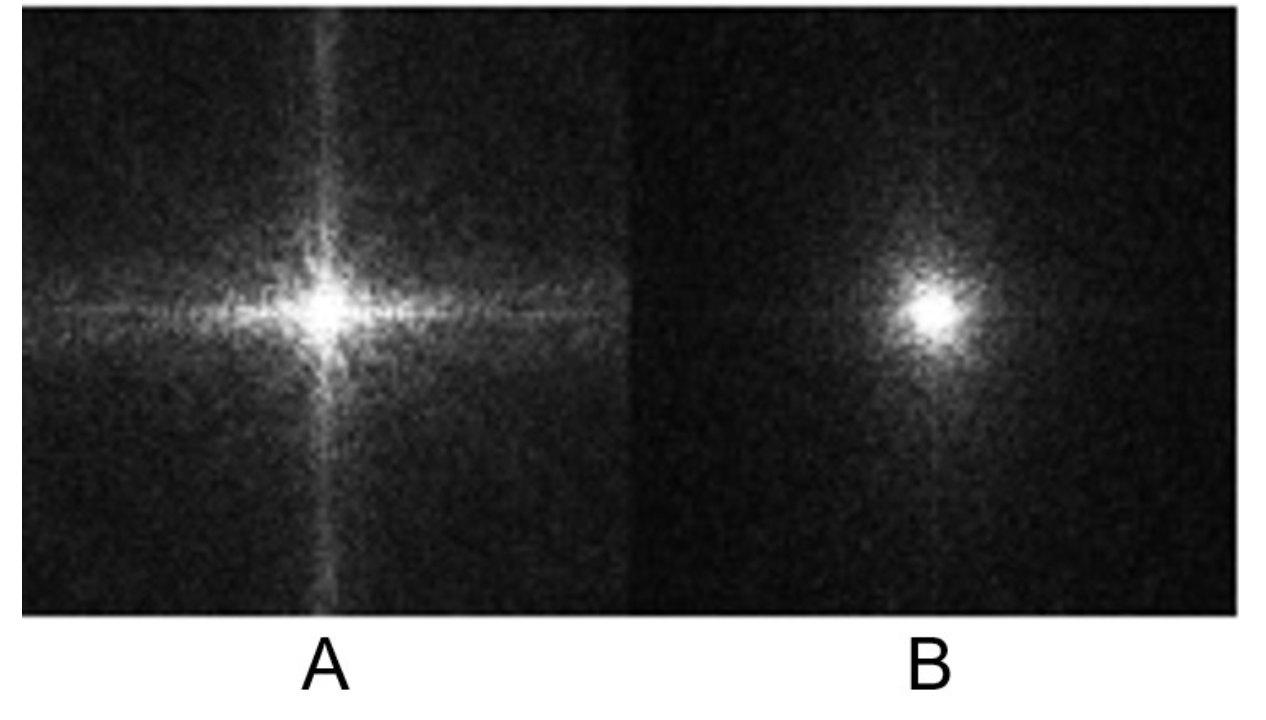
\includegraphics[width=0.5\linewidth]{figures/spectra.png}
\end{center}
\begin{itemize}[leftmargin=1.8em]
  \choice A
  \choice B
\end{itemize}
\closequestion

\questiontitle{Image Aggregation}
What are examples for image aggregation? (Multiple choices possible.)
\begin{itemize}[leftmargin=1.8em]
  \choice Panorama imaging
  \choice High-Dynamic Range (HDR) imaging
  \choice Single-shot object detection
\end{itemize}
\closequestion

\questiontitle{Gradient Field Properties}
Which of the following statements is correct? (Multiple choices possible.)
\begin{itemize}[leftmargin=1.8em]
  \choice The gradient field of an image has zero curl.
  \choice The gradient field of an image is a conservative vector field.
  \choice After processing the gradient field, the corresponding image can always be reconstructed by integration.
  \choice The divergence of the gradient field is the Laplacian of the corresponding image.
\end{itemize}
\closequestion


% ==========================================================
\section{Optical Flow}
% ==========================================================

\questiontitle{Sparse Optical Flow Assumptions}
What assumptions are made for sparse optical flow estimations (e.g., Lucas-Kanade)? (Multiple choices possible.)
\begin{itemize}[leftmargin=1.8em]
  \choice Spatial Coherence
  \choice Color/Brightness Consistency
  \choice Smooth Flow Fields
\end{itemize}
\closequestion

\questiontitle{Lucas-Kanade: Large Displacements}
How do you compute optical flow that is larger than one pixel in the Lucas-Kanade optical flow approach?
\begin{itemize}[leftmargin=1.8em]
  \choice That is not possible. You need to apply a dense optical flow approach instead.
  \choice You increase the considered neighborhood pixels to get more equations.
  \choice You compute the optical flow at multiple resolutions.
\end{itemize}
\closequestion

\questiontitle{Lucas-Kanade vs.\ Horn-Schunck}
Which statement best describes the main difference between the Lucas-Kanade and Horn-Schunck optical flow method?
\begin{itemize}[leftmargin=1.8em]
  \choice Lucas-Kanade estimates optical flow by solving a local least-squares problem, while Horn-Schunck estimates optical flow by minimizing a global energy function with a smoothness constraint.
  \choice Horn-Schunck works only for small motion, while Lucas-Kanade handles large displacement without modification.
  \choice Lucas-Kanade produces dense optical flow, while Horn-Schunck produces sparse optical flow only by default.
  \choice Lucas-Kanade enforces global smoothness, while Horn-Schunck estimates motion independently per pixel.
\end{itemize}
\closequestion

\questiontitle{Stereo Optical Flow and Disparity}
For a static rectified stereo-camera system and a static scene, the dense optical flow field of a recorded stereo pair correlates to a disparity map. (True/False)
\begin{itemize}[leftmargin=1.8em]
  \choice True
  \choice False
\end{itemize}
\closequestion

\questiontitle{Deep Learning-Based Optical Flow}
Which of the following statements about deep learning-based optical flow estimation are correct? (Multiple choices possible.)
\begin{itemize}[leftmargin=1.8em]
  \choice Encoder-decoder architectures (e.g., U-Net-like networks) are commonly used to produce dense optical flow fields.
  \choice Convolutional neural networks for optical flow inference typically require explicit computation of image gradients.
  \choice Deep learning methods estimate optical flow by learning a direct mapping from pairs of images to flow fields.
\end{itemize}
\closequestion


% ==========================================================
\section{Deep Learning, Recognition, and Detection}
% ==========================================================

\questiontitle{SIFT Scale Invariance}
SIFT is not scale invariant. (True/False)
\begin{itemize}[leftmargin=1.8em]
  \choice True
  \choice False
\end{itemize}
\closequestion

\questiontitle{Scale Invariance in CNNs}
For model-based feature extraction, image pyramids are used to achieve scale invariance. What is used to achieve this in CNNs?
\begin{itemize}[leftmargin=1.8em]
  \choice Convolution
  \choice Pooling and downsampling
  \choice ReLU
\end{itemize}
\closequestion

\questiontitle{ResNet vs.\ Human Performance}
ResNet can achieve a better top-5-error rate than humans. (True/False)
\begin{itemize}[leftmargin=1.8em]
  \choice True
  \choice False
\end{itemize}
\closequestion

\questiontitle{ReLU Output}
What is ReLU$(-1234)$?

Answer: \answerline{3cm}
\closequestion

\questiontitle{ReLU Activation Purpose}
In a Convolutional Neural Network (CNN), the Rectified Linear Unit (ReLU) activation function $f(x)=\max(0,x)$ is primarily used to:
\begin{itemize}[leftmargin=1.8em]
  \choice Introduce non-linearity and help mitigate the vanishing gradient problem.
  \choice Normalize pixel values to a range between 0 and 1.
  \choice Reduce the spatial dimensions of feature maps.
  \choice Compute gradient orientations for feature descriptors.
\end{itemize}
\closequestion

\questiontitle{Max-Pooling Purpose}
What is the reason for max-pooling in CNNs used for image classification?
\begin{itemize}[leftmargin=1.8em]
  \choice It averages feature responses and therefore it is more robust.
  \choice It provides higher spatial accuracy for feature positions.
  \choice It provides a large response regardless of the exact feature position.
\end{itemize}
\closequestion

\questiontitle{CNN Activation Layer Resolution}
Given a Convolutional Neural Network using filter kernels of $7\times7$: What is the resolution of the 3rd activation layer if no pooling is applied, and if the input image resolution is $32\times32$? (Type in only one dimension, e.g., 32 for $32\times32$.)

Answer: \answerline{3cm}
\closequestion

\questiontitle{Transposed Convolution Output Resolution}
Your input image is $4\times4$ and your kernel is $3\times3$. What is the resolution of the output image after transposed convolution if your stride is 2 and padding is 1?

Note: if your output resolution is $A\times A$, type in only $A$.

Answer: \answerline{3cm}
\closequestion

\questiontitle{CNN Architecture for Segmentation}
What is a practical CNN architecture for segmentation tasks?
\begin{itemize}[leftmargin=1.8em]
  \choice A CNN with conv-layers of same resolution (without down-sampling).
  \choice A conventional CNN where conv-layers are down-sampled.
  \choice A CNN where conv-layers are down- and up-sampled inside the network.
\end{itemize}
\closequestion

\questiontitle{U-Net Skip Connections}
In a U-Net architecture for semantic segmentation, what is/are the primary purpose(s) of skip connections between corresponding encoder and decoder layers? (Multiple choices possible.)
\begin{itemize}[leftmargin=1.8em]
  \choice Mid-level representations are often formed by clustering low-level features before classification.
  \choice To preserve high-resolution spatial information lost during down-sampling.
  \choice To reduce the number of trainable parameters.
  \choice To introduce non-linearity into the decoder.
  \choice To allow the network to bypass the bottleneck layer entirely.
\end{itemize}
\closequestion

\questiontitle{Instance Segmentation}
Instance segmentation gives you a pixel-to-class assignment, but it is not possible to differentiate between different instances of the same class. (True/False)
\begin{itemize}[leftmargin=1.8em]
  \choice True
  \choice False
\end{itemize}
\closequestion

\questiontitle{Scale-Depth Ambiguity}
What is the standard option to overcome the scale-depth ambiguity problem when estimating depth-maps with CNNs?
\begin{itemize}[leftmargin=1.8em]
  \choice Assume smoothness in the gradients of the reconstructed depth map.
  \choice Consider the global scene scale in the loss function.
  \choice Segment the scene into different object-clusters first, and then estimate their depth values independently.
  \choice Assume smoothness in surface normals of the reconstructed depth map.
\end{itemize}
\closequestion

\questiontitle{Scale-Invariant Loss for Depth Prediction}
What is the primary purpose of using a scale-invariant loss function for monocular depth prediction?
\begin{itemize}[leftmargin=1.8em]
  \choice To improve the accuracy of surface normal prediction.
  \choice To eliminate the need for ground truth depth data.
  \choice To reduce computation time during training.
  \choice To account for the fundamental scale-depth ambiguity in single-image depth estimation.
\end{itemize}
\closequestion

\questiontitle{Neural Networks for Depth Reconstruction}
How can neural networks be used for depth reconstruction? (Multiple choices possible.)
\begin{itemize}[leftmargin=1.8em]
  \choice Fully connected layers can be used to learn the cost function.
  \choice Autoencoders (U-Nets) can be used for end-to-end learning.
  \choice U-Nets can be used to learn epipolar constraints.
  \choice CNNs can be used for feature extraction.
\end{itemize}
\closequestion

\questiontitle{Cost-Volumes in PSMNet}
Cost-Volumes in PSMNet (and other models) are used for \dots (Multiple choices possible.)
\begin{itemize}[leftmargin=1.8em]
  \choice \dots extracting features from multiple views at multiple scales with spatial pyramid pooling (SPP).
  \choice \dots computing matching costs with a 3D CNN.
  \choice \dots concatenating features from multiple views at all possible disparities.
\end{itemize}
\closequestion

\questiontitle{ResNet Layers for Depth from Defocus}
Can individual conv-layers of ResNet be used for Depth from Defocus estimations? (Multiple choices possible.)
\begin{itemize}[leftmargin=1.8em]
  \choice Yes, because they provide feature saliency information that are proportional to focus.
  \choice Yes, but only for uniform regions.
  \choice No, because ResNet does not provide per-pixel information.
  \choice Yes, but only for non-uniform regions.
  \choice No, because ResNet is a model used for classification.
\end{itemize}
\closequestion

\questiontitle{Learned Filter Kernels in CNNs}
For which conv layers of a CNN do you expect to find learned filter kernels that approximate Gaussians (assuming classical training databases, such as ImageNet)?
\begin{itemize}[leftmargin=1.8em]
  \choice Mid-level conv layers.
  \choice High-level conv layers.
  \choice Low-level conv layers.
\end{itemize}
\closequestion

\questiontitle{Vision Transformers}
For Vision Transformers \dots (Multiple choices possible.)
\begin{itemize}[leftmargin=1.8em]
  \choice \dots only the decoder part is usually used.
  \choice \dots linear projections of reshaped image patches + positional embeddings are usually used as input.
  \choice \dots only the encoder part is usually used.
  \choice \dots both encoder and decoder are usually used.
\end{itemize}
\closequestion

\questiontitle{Neural Radiance Fields: Inverse Problem}
Neural Radiance Fields solve an inverse problem. (True/False)
\begin{itemize}[leftmargin=1.8em]
  \choice True
  \choice False
\end{itemize}
\closequestion

\questiontitle{NeRF Architecture}
The architecture behind classical Neural Radiance Fields (NeRFs) is \dots
\begin{itemize}[leftmargin=1.8em]
  \choice \dots a CNN.
  \choice \dots a transformer.
  \choice \dots a fully connected network.
  \choice \dots a U-Net.
\end{itemize}
\closequestion

\questiontitle{NeRF Output}
What does a Neural Radiance Field (NeRF) model output for a given 3D point and viewing direction?
\begin{itemize}[leftmargin=1.8em]
  \choice Vertex coordinates and texture.
  \choice Depth and surface normal.
  \choice Occupancy probability and gradient.
  \choice Volume density and RGB color.
\end{itemize}
\closequestion

\questiontitle{NeRF with Binary Opacity}
If you would condition the opacity solutions of Neural Radiance Fields to be binary, what kind of scenes would you still be able to represent with it? (Multiple choices possible.)
\begin{itemize}[leftmargin=1.8em]
  \choice Scenes with anisotropic reflections.
  \choice Scenes with refractions.
  \choice Scenes with specular reflections.
  \choice Scenes with isotropic reflections.
  \choice Scenes with diffuse reflections.
\end{itemize}
\closequestion

\questiontitle{Image--Text Correlation Model}
What model can be used directly to learn correlations of images and text descriptions?
\begin{itemize}[leftmargin=1.8em]
  \choice Grad-CAM
  \choice CLIP
  \choice YOLO
  \choice ResNET
\end{itemize}
\closequestion

\questiontitle{Large Multi-Modal Models}
Which of the following statements about Large Multi-Modal Models (LMMs) are correct? (Multiple choices possible.)
\begin{itemize}[leftmargin=1.8em]
  \choice LMMs can be used for high-level vision tasks (e.g., reasoning) but may struggle with precise low-level tasks such as precise spatial estimations.
  \choice LMMs suffer from poor generalization to novel visual concepts due to overfitting on language data.
  \choice LMMs suffer from hallucination of visual content not present in images.
  \choice LMMs can only perform tasks for which all input modalities are present at inference time.
\end{itemize}
\closequestion

\questiontitle{Non-Maximum Suppression in YOLO}
Non-maximum suppression in YOLO \dots
\begin{itemize}[leftmargin=1.8em]
  \choice \dots removes bounding boxes that are too different.
  \choice \dots removes bounding boxes that are too similar.
\end{itemize}
\closequestion

\questiontitle{Region Proposal Network in Faster R-CNN}
What is the primary function of the Region Proposal Network (RPN) in Faster R-CNN?
\begin{itemize}[leftmargin=1.8em]
  \choice To compute the loss for objectness.
  \choice To perform bounding box regression.
  \choice To propose regions that likely contain objects.
  \choice To classify objects into specific categories.
\end{itemize}
\closequestion

\questiontitle{Intersection over Union}
The intersection over union of the two bounding boxes (red and blue) shown below is \dots (Select all that apply.)
\begin{center}
  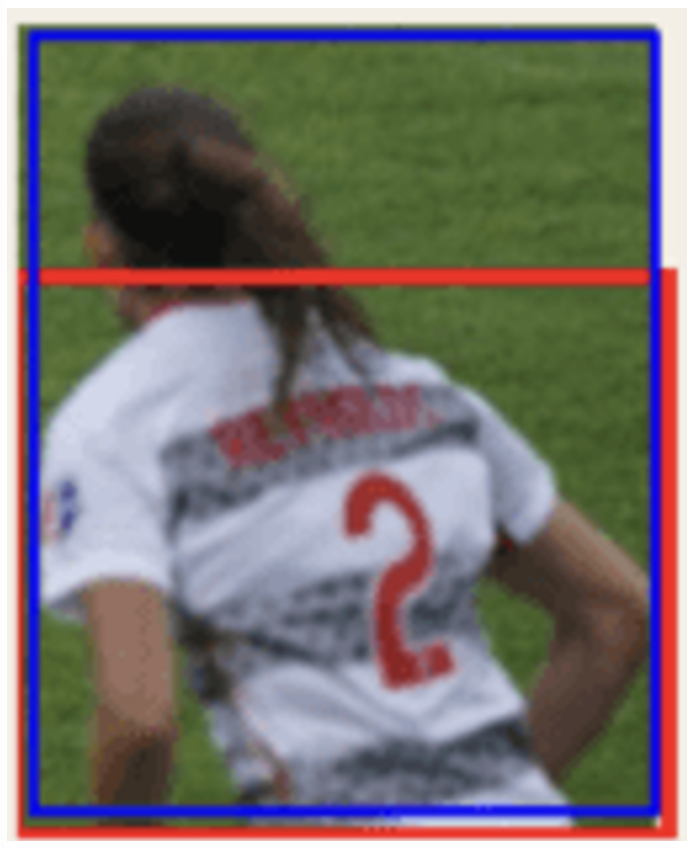
\includegraphics[width=0.4\linewidth]{figures/boxes.png}
\end{center}
\begin{itemize}[leftmargin=1.8em]
  \choice $< 0.5$
  \choice $> 0.5$
  \choice $> 1$
  \choice $< 0$
  \choice $< 1$
\end{itemize}
\closequestion

\questiontitle{Precision}
A detector produces the following results for a class: TP$=80$, FP$=20$, FN$=40$. What is the precision?

Answer: \answerline{3cm}
\closequestion

\questiontitle{Average Precision and Precision--Recall Curve}
Let's assume your precision-recall curve is smooth; then an average precision of 0.5 indicates a relationship between recall and precision that is \dots
\begin{itemize}[leftmargin=1.8em]
  \choice \dots cubic.
  \choice \dots constant.
  \choice \dots quadratic.
  \choice \dots linear.
\end{itemize}
\closequestion

\questiontitle{K-Means Determinism}
K-means clustering is deterministic. (True/False)
\begin{itemize}[leftmargin=1.8em]
  \choice True
  \choice False
\end{itemize}
\closequestion

\questiontitle{Training Dataset Roles}
Correlate the different parts of a training dataset with its functionality. Match each dataset split (left) to its role (right):

\medskip
\begin{tabular}{ll}
  \textbf{Test data} & \answerline{5cm} \\[6pt]
  \textbf{Training data} & \answerline{5cm} \\[6pt]
  \textbf{Validation data} & \answerline{5cm}
\end{tabular}

\medskip
Roles: \emph{Determine final accuracy} \quad \emph{Train model parameters} \quad \emph{Tune hyperparameters}
\closequestion

\questiontitle{Event Cameras}
Event cameras differ fundamentally from conventional frame-based cameras. Which of the following statements about event cameras are correct? (Multiple choices possible.)
\begin{itemize}[leftmargin=1.8em]
  \choice Event cameras inherently suffer from motion blur when observing fast-moving objects.
  \choice Event cameras generally offer higher temporal resolution and lower latency than frame-based cameras.
  \choice Event cameras asynchronously report changes in pixel intensity rather than capturing full image frames at fixed intervals.
  \choice Event cameras require significantly more bandwidth than conventional cameras because they continuously stream all pixel values.
  \choice Each event typically encodes the pixel location, timestamp, and the brightness change.
\end{itemize}
\closequestion

\questiontitle{CNN Trainable Parameters}
A convolution layer is designed with input volume of $32\times 32\times 3$ and has 16 filters, each of size $3\times 3\times 3$. Assuming no bias terms are used, how many trainable parameters are in this convolutional layer?

Answer: \answerline{3cm}
\closequestion

\questiontitle{Convolution Output Value}
An image patch is given by
\[
I = \begin{pmatrix}
1 & 2 & 1\\
0 & 0 & 0\\
-1 & -2 & -1
\end{pmatrix}
\]
and the convolution kernel is
\[
h = \begin{pmatrix}
1 & 0 & -1\\
2 & 0 & -2\\
1 & 0 & -1
\end{pmatrix}.
\]
What is the output value at the center pixel after convolution (assume valid convolution, no padding)?

Answer: \answerline{3cm}
\closequestion

\questiontitle{Capturing Digital Images: Multiple Statements}
Select all statements that are correct with respect to capturing digital images. (Multiple choices possible.)
\begin{itemize}[leftmargin=1.8em]
  \choice Color values in an RGB image measured through a Bayer filter are typically obtained by interpolation from neighboring subpixels.
  \choice A higher signal-to-noise ratio generally results in more reliable intensity measurements.
  \choice CMOS and CCD sensors measure the number of photons arriving at each pixel location over exposure time.
  \choice Sensor noise has a stronger relative impact in dark image regions than in bright regions.
  \choice In a Bayer filter pattern, each pixel directly measures all three color channels (R, G, and B).
\end{itemize}
\closequestion

\questiontitle{Autoencoder vs.\ U-Net Differences}
\repeatnote

What are the differences between simple autoencoders and U-Nets used for segmentation?
\begin{itemize}[leftmargin=1.8em]
  \choice A simple autoencoder has an encoder and a decoder, while a U-Net has only an encoder.
  \choice A U-Net has an encoder and a decoder, while a simple autoencoder has only an encoder.
  \choice U-Nets have skip connections.
\end{itemize}
\closequestion

\questiontitle{Why U-Nets Excel at Segmentation}
\repeatnote

U-Nets are better suited for segmentation tasks than unconnected autoencoders because \dots
\begin{itemize}[leftmargin=1.8em]
  \choice \dots of their additional pooling.
  \choice \dots of their additional convolutions.
  \choice \dots of their additional skip-connections.
  \choice \dots of their additional transposed convolutions.
\end{itemize}
\closequestion

\questiontitle{Traditional Model-Based Classification Pipeline}
In a traditional model-based classification pipeline (e.g., using handcrafted features like SIFT), which of the following statements are true?
\begin{itemize}[leftmargin=1.8em]
  \choice It typically involves steps such as feature detection, descriptor extraction, and clustering.
  \choice Feature detectors are manually designed and remain fixed (e.g., edge, corner, and blob detectors).
  \choice Mid-level representations are often formed by clustering low-level features before classification.
  \choice The feature extraction kernels are learned automatically from labeled training data.
  \choice It requires no preprocessing or invariance handling (e.g., scale or rotation invariance).
\end{itemize}
\closequestion


% ==========================================================
%  ANSWER KEY
% ==========================================================
\newpage
\section*{Answer Key}

\begin{enumerate}[label=\textbf{Q\arabic*.}, leftmargin=3em, itemsep=4pt]
  % Capturing Digital Images (Q1–Q11)
  \item \textbf{a, c}
  \item $20$\,mm
  \item $128$\,mm
  \item \textbf{c}
  \item \textbf{a, c}
  \item \textbf{a}
  \item \textbf{a}
  \item \textbf{a, c, e}
  \item \textbf{d}
  \item \textbf{a, b, c}
  \item \textbf{b} (False)
  % Multi-View Geometry (Q12–Q30)
  \item \textbf{a, b}
  \item \textbf{a} (True)
  \item \textbf{c, e, f}
  \item \textbf{b}
  \item \textbf{b} (False)
  \item $1$
  \item \textbf{a, b}
  \item \textbf{b} (False)
  \item $120$
  \item $111$
  \item \textbf{b, d}
  \item \textbf{c}
  \item $72$ (7 points, 2 views)
  \item $6$
  \item \textbf{a} (27)
  \item \textbf{b}
  \item \textbf{b}
  \item \textbf{a} (True)
  \item \textbf{a} (True)
  % Digital Image Processing (Q31–Q50)
  \item \textbf{d}
  \item \textbf{a, c, d, e}
  \item \textbf{b} (False)
  \item \textbf{b} (False)
  \item \textbf{c}
  \item \textbf{c}
  \item \textbf{c}
  \item $5$
  \item \textbf{d}
  \item \textbf{a}
  \item \textbf{b} (False)
  \item $2$
  \item \textbf{e}
  \item \textbf{d}
  \item \textbf{e} (20)
  \item \textbf{a, c}
  \item \textbf{a}
  \item \textbf{a}
  \item \textbf{a, b}
  \item \textbf{a, b, d}
  % Optical Flow (Q51–Q55)
  \item \textbf{a, b}
  \item \textbf{c}
  \item \textbf{a}
  \item \textbf{a} (True)
  \item \textbf{a, c}
  % Deep Learning, Recognition, and Detection (Q56–Q93)
  \item \textbf{b} (False)
  \item \textbf{b}
  \item \textbf{a} (True)
  \item $0$
  \item \textbf{a}
  \item \textbf{c}
  \item $14$
  \item $7$
  \item \textbf{c}
  \item \textbf{b}
  \item \textbf{b} (False)
  \item \textbf{b}
  \item \textbf{d}
  \item \textbf{a, b, d}
  \item \textbf{b, c}
  \item \textbf{a, d}
  \item \textbf{c}
  \item \textbf{b, c}
  \item \textbf{a} (True)
  \item \textbf{c}
  \item \textbf{d}
  \item \textbf{d, e}
  \item \textbf{b}
  \item \textbf{a, c}
  \item \textbf{b}
  \item \textbf{c}
  \item \textbf{b, e}
  \item $0.8$
  \item \textbf{d}
  \item \textbf{b} (False)
  \item Test data $\to$ Determine final accuracy;\ Training data $\to$ Train model parameters;\ Validation data $\to$ Tune hyperparameters
  \item \textbf{b, c, e}
  \item $432$
  \item $0$
  \item \textbf{a, b, c, d}
  \item \textbf{c}
  \item \textbf{c}
  \item \textbf{a, b, c}
\end{enumerate}


\end{document}
